% !TeX encoding = UTF-8
% !TeX program = xelatex
% !TeX spellcheck = en_US

\documentclass[degree=project,degree-type=project,cjk-font=noto]{thuthesis}
\usepackage{mathtools}
\usepackage{tikz}
\usetikzlibrary{shapes,arrows}
\usepackage[autosize]{dot2texi}
% Syntax Highlighting in LaTeX, need pygments
% Must build with xelatex -shell-escape -enable-8bit-chars.
\usepackage{minted}
% https://tex.stackexchange.com/a/112573
\usepackage{tcolorbox}
\usepackage{etoolbox}
\BeforeBeginEnvironment{minted}{\begin{tcolorbox}}%
\AfterEndEnvironment{minted}{\end{tcolorbox}}%
% color for minted
\definecolor{friendlybg}{HTML}{f0f0f0}


% 论文基本配置,加载宏包等全局配置
\thusetup{
    output = electronic,
    title  = {实验一},
    author  = {肖文韬},
    studentid = {2020214245},
    major = {电子信息(计算机技术)},
    email = {xwt20@mails.tsinghua.edu.cn},
    course = {密码学与网络安全},
    include-spine = false,
}


\usepackage{float}
\usepackage[sort]{natbib}
\bibliographystyle{thuthesis-numeric}
\graphicspath{{figures/}}


\setlist[enumerate,1]{label=\arabic*.}
\setlist[enumerate,2]{label=(\alph*)}
\setlist[enumerate,3]{label=\roman*.}
\setlist[enumerate,4]{label=\greek*}

\newcommand*\justify{%
  \fontdimen2\font=0.4em% interword space
  \fontdimen3\font=0.2em% interword stretch
  \fontdimen4\font=0.1em% interword shrink
  \fontdimen7\font=0.1em% extra space
  \hyphenchar\font=`\-% allowing hyphenation
}

\renewcommand{\texttt}[1]{%
  \begingroup
  \ttfamily
  \begingroup\lccode`~=`/\lowercase{\endgroup\def~}{/\discretionary{}{}{}}%
  \begingroup\lccode`~=`[\lowercase{\endgroup\def~}{[\discretionary{}{}{}}%
  \begingroup\lccode`~=`.\lowercase{\endgroup\def~}{.\discretionary{}{}{}}%
  \catcode`/=\active\catcode`[=\active\catcode`.=\active
  \justify\scantokens{#1\noexpand}%
  \endgroup
}


\begin{document}

% 封面
\maketitle

\frontmatter
% % !TeX root = ../thuthesis-example.tex

% 中英文摘要和关键字

\begin{abstract}
  论文的摘要是对论文研究内容和成果的高度概括。摘要应对论文所研究的问题及其研究目
  的进行描述,对研究方法和过程进行简单介绍,对研究成果和所得结论进行概括。摘要应
  具有独立性和自明性,其内容应包含与论文全文同等量的主要信息。使读者即使不阅读全
  文,通过摘要就能了解论文的总体内容和主要成果。

  论文摘要的书写应力求精确、简明。切忌写成对论文书写内容进行提要的形式,尤其要避
  免“第 1 章……;第 2 章……;……”这种或类似的陈述方式。

  本文介绍清华大学论文模板 \thuthesis{} 的使用方法。本模板符合学校的本科、硕士、
  博士论文格式要求。

  本文的创新点主要有:
  \begin{itemize}
    \item 用例子来解释模板的使用方法;
    \item 用废话来填充无关紧要的部分;
    \item 一边学习摸索一边编写新代码。
  \end{itemize}

  关键词是为了文献标引工作、用以表示全文主要内容信息的单词或术语。关键词不超过 5
  个,每个关键词中间用分号分隔。(模板作者注:关键词分隔符不用考虑,模板会自动处
  理。英文关键词同理。)

  % 关键词用“英文逗号”分隔
  \thusetup{
    keywords = {TeX, LaTeX, CJK, 模板, 论文},
  }
\end{abstract}

\begin{abstract*}
  An abstract of a dissertation is a summary and extraction of research work
  and contributions. Included in an abstract should be description of research
  topic and research objective, brief introduction to methodology and research
  process, and summarization of conclusion and contributions of the
  research. An abstract should be characterized by independence and clarity and
  carry identical information with the dissertation. It should be such that the
  general idea and major contributions of the dissertation are conveyed without
  reading the dissertation.

  An abstract should be concise and to the point. It is a misunderstanding to
  make an abstract an outline of the dissertation and words ``the first
  chapter'', ``the second chapter'' and the like should be avoided in the
  abstract.

  Key words are terms used in a dissertation for indexing, reflecting core
  information of the dissertation. An abstract may contain a maximum of 5 key
  words, with semi-colons used in between to separate one another.

  \thusetup{
    keywords* = {TeX, LaTeX, CJK, template, thesis},
  }
\end{abstract*}


% 目录
% \tableofcontents

% 插图和附表清单
% \listoffiguresandtables
% \listoffigures           % 插图清单

% 正文部分
\mainmatter

\chapter{实验介绍}
AES加密算法是迭代型分组密码算法,涉及4种操作:字节替代、行移位、列混合和轮密钥加。
本次实验中密钥长度和分组长度都为128比特,加密轮数为10轮。
实验使用 Rust 语言实现 AES128 的加密解密操作。

实验目的:

\begin{enumerate}
    \item 熟练掌握AES加密算法的理论
    \item 学习 rust 语言的基本用法
\end{enumerate}

实验平台:

\begin{enumerate}
    \item rust 语言
    \item Arch Linux (不依赖具体操作系统,rust 亦可在 windows/macOS 上使用)
\end{enumerate}

\chapter{实验内容}

\section{字节替代变换和逆字节替代变换}

    根据16×16的字节替代矩阵和逆替代矩阵,对于每个字节,将其前4bit作为横坐标,后4bit作为纵坐标,使用下方替代矩阵对应位置的字节进行替代。完成对一个长文本的字节替代变换和逆字节替代变换,对于不足16字符的输入需要补位,为了方便之后的加解密,16字节的文本应转换为4×4的字节矩阵。

{\heiti 解:}

因为 AES128 是作用于块大小为 128 bits 的块加密算法。
所以本题首先需要实现将明文消息分块,并且对于最后一块不足 16 字节时进行补位。
再对每一块进行字节替代,再进行逆字节替代。
最后进行逆补位得到原文。

\subsection{补位}

  \begin{minted}[texcomments,tabsize=2,fontsize=\normalsize,style=friendly,bgcolor=friendlybg]{rust}
fn pad(states: &mut Vec<u8>) -> () {
  let mut pad_size = states.len() % BLOCK_SIZE;
  if pad_size != 0 {
      pad_size = BLOCK_SIZE - pad_size;
  }
  states.extend(vec![PAD_BYTE; pad_size]);
}
  \end{minted}

其中 \texttt{PAD\_BYTE} 为 $0$,即用 $0$ 来补位,\texttt{BLOCK\_SIZE} 为 $16$ 字节,即 $128$ bits。

\subsection{字节替代}

  \begin{minted}[texcomments,tabsize=2,fontsize=\footnotesize,style=friendly,bgcolor=friendlybg]{rust}
fn sub_bytes(states: &mut Vec<u8>) -> () {
  for idx in 0..states.len() {
      let b = states[idx];
      states[idx] = SBOX[(b >> 4) as usize][(b & 0x0f) as usize];
  }
}
  \end{minted}

其中 SBOX 是提前给定的,SBOX 就是一个二维数组,第一维就是字节的高 4 位,第二维就是字节的低 4 位,具体的 SBOX 定义见源代码/实验书。

\subsection{逆字节替代}

  \begin{minted}[texcomments,tabsize=2,fontsize=\footnotesize,style=friendly,bgcolor=friendlybg]{rust}
fn inv_sub_bytes(states: &mut Vec<u8>) -> () {
    for idx in 0..states.len() {
        let b = states[idx];
        states[idx] = INV_SBOX[(b >> 4) as usize][(b & 0x0f) as usize];
    }
}
  \end{minted}

INV\_SBOX 就是根据 SBOX 对应的逆替换表。

\subsection{逆补位}

  \begin{minted}[texcomments,tabsize=2,fontsize=\footnotesize,style=friendly,bgcolor=friendlybg]{rust}
fn unpad(states: &mut Vec<u8>) -> () {
    let blocks = states.chunks_mut(BLOCK_SIZE);
    let last_block: &mut [u8] = blocks.last().unwrap();
    let padding_len = BLOCK_SIZE - match last_block.iter().position(
        |&x| x == PAD_BYTE) {
        Some(pos) => pos,
        None => BLOCK_SIZE,
    };
    for _ in 0..padding_len {
        states.remove(states.len() - 1);
    }
}
  \end{minted}

逆补位稍微复杂一点,首先需要在逆变换后的补位长度,然后将补位部分截断即可。

\subsection{运行结果}

\begin{figure}[h]
\centering%
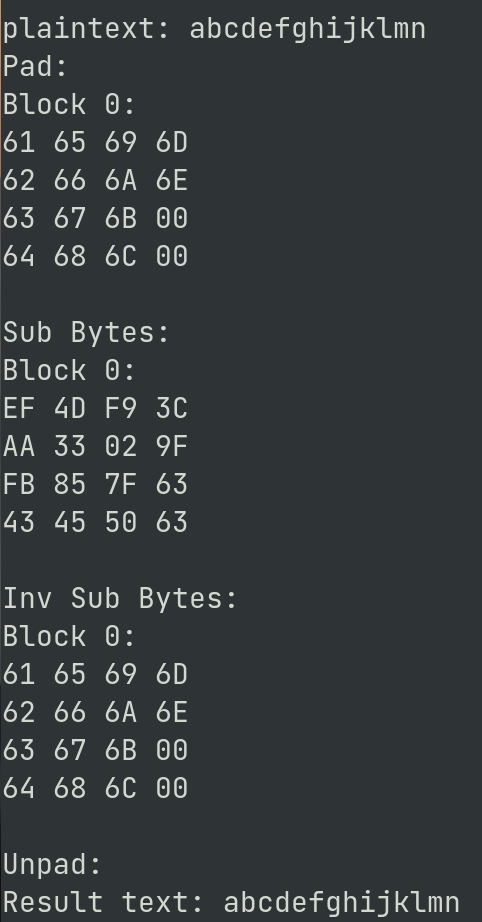
\includegraphics[width=.4\linewidth]{aes_t1.png}
  \caption{字节替换运行结果}
  \label{fig:t1}
\end{figure}

本题使用字符串'abcdefghijklmn'作为输入,完成字符串的补位、转码、字节替代、逆字节替代、转码、去补位,输出每一步的结果。
运行结果如图~\ref{fig:t1}所示。

\section{行移位变换和逆行移位变换,列混合和逆列混合}

编写对4×4字节矩阵的行移位变换和逆行移位变换代码。编写对4×4字节矩阵的列混合和逆列混合代码,列混合需要使用x乘法 (xtime)。

\subsection{行移位变换}

行移位就是将每一块(block)用状态矩阵(state)表示,然后对每一行做一些简单的循环左移运算。
具体的,第一行不移位,第二行循环左移一位,第三行循环左移两位,第四行循环左移三位。

  \begin{minted}[texcomments,tabsize=2,fontsize=\footnotesize,style=friendly,bgcolor=friendlybg]{rust}
fn shift_rows(states: &mut Vec<u8>) -> () {
    let blocks = states.chunks_mut(BLOCK_SIZE);
    for state in blocks {
        let mut temp: u8;
        // row 1
        temp = state[1];
        state[1] = state[5];
        state[5] = state[9];
        state[9] = state[13];
        state[13] = temp;
        // row 2
        temp = state[2];
        state[2] = state[10];
        state[10] = temp;
        temp = state[6];
        state[6] = state[14];
        state[14] = temp;
        // row 3
        temp = state[15];
        state[15] = state[11];
        state[11] = state[7];
        state[7] = state[3];
        state[3] = temp;
    }
}
  \end{minted}

\subsection{列混合}

在列混合中,状态矩阵中的每一个字节都可以看作是 $GF(2^8)$ 有限域上的多项式,且最高项次数不超过 $7$。
在 $GF(2^8)$ 上乘以另外一个模多项式 $c(x)$ 再取模可以写作一个矩阵运算(由 $GF(2^8)$ 上定义的乘法实现的)。
对于 输入多项式 $a(x)$,乘以模多项式 $c(x) = '03'x^3+'01'x^2+'01'x+'02'$ 可以表示为:
\begin{align}
  \begin{split}
    b(x) &= c(x) \otimes a(x) \\
    &= \begin{bmatrix}
      02 & 03 & 01 & 01 \\
      01 & 02 & 03 & 01 \\
      01 & 01 & 02 & 03 \\
      03 & 01 & 01 & 02
    \end{bmatrix} \begin{bmatrix}
      a_0 \\
      a_1 \\
      a_2 \\
      a_3
    \end{bmatrix}
  \end{split}
\end{align}

注意 $GF(2^8)$ 上的加法就是异或运算。
同时,$GF(2^8)$ 上一个多项式乘以任意多项式(任意常数)都可以归约为乘以常数 '02' (也就是多项式 $x$,也叫做 x 乘法)和 '01' (那就是本身啦)。
例如,上面矩阵的结果中,有以下推导:

\begin{align*}
    b_0 &= '02' \cdot a_0 + '03' \cdot a_1 + '01' \cdot a_2 + '01' \cdot a_3 \\
    '02' \cdot a_0 + a_1 \cdot ('01' + '02') + a_2 + a_3 \\
    &= (a_0 + a_1) \cdot '02' + a_1 + a_2 + a_3 \\
    &= (a_0 + a_1) \cdot '02' + a_0 + a_0 + a_1 + a_2 + a_3
\end{align*}
其中 $GF(2^8)$ 上的加法运算就是二进制的逐位异或(xor),这里面利用了一些异或的性质就不再展开了,比较容易自己推导出来。

x 乘法(xtime)的实现代码如下:

  \begin{minted}[texcomments,tabsize=2,fontsize=\footnotesize,style=friendly,bgcolor=friendlybg]{rust}
fn xtime(b: u8) -> u8 {
    let c;
    if (b & 0x80) != 0 {
        c = (b << 1) ^ 0x1b;
    } else {
        c = b << 1;
    };
    c
}
  \end{minted}

代码看起来是简单,不过推导起来有不少步骤。
首先 $GF(2^8)$ 上的数,就是对应一个多项式,例如 $'1B' (0b0001\_1011)$ 就对应多项式 $x^4 + x^3 + x + 1$。
两个 $GF(2^8)$ 上的数相乘,就是对应他们的多项式在 $\mathbb{R}$ 上的普通乘法。
比如 x 乘法就是将数乘以多项式 $x$ (也就是 '02'),例如 $'1B' \cdot '02' = (x^4 + x^3 + x + 1) x = x^5 + x^4 + x^2 + x = 0b0011\_0110 = '54'$,其实就是二进制左移一位.
还有就是取模运算也不用于 $\mathbb{R}$ 上的取模,$GF(2^8)$ 上的取模笼统地来说就是用异或实现的除法。
举个例子,计算 $'B3' \cdot '02' \;(\bmod\; '11B') = 0b1011\_0011 \ll 2 \;(\bmod\; 0b1\_0001_1011) = 0b1\_0110\_0110 \;(\bmod 0b1\_0001\_1011)$ 过程如下:

{\tt
{\noindent-------------}\\
\phantom{0 }1 0110 0110 (mod) 1 0001 1011 \\
\textasciicircum\phantom{ }1 0001 1011 \\
------------- \\
\phantom{0 }0 0111 1101
}

其中上面的 $\textasciicircum$ 就是异或运算。
又因为 $GF(2^8)$ 最高阶就是 $x^7$ (二进制的最高位), 而模多项式 $'11B'$ 对应的最高阶是 $x^8$,也就是多一位。
所以 x 乘法的被乘出只有两种可能:(1)最高位是 $0$,则左移一位也不会超过 $'11B'$,所以取模后仍未原数,(2)最高位是 $1$,则左移一位后可能会大于模多项式,这时候我们需要使用上述取模的过程,与模多项式进行一次异或运算。
综上,这个代码逻辑就很好理解了。

有了 x 乘法,我们就可以得出乘以任意多项式的算法了,下面的代码就是列混淆的最终实现。

  \begin{minted}[texcomments,tabsize=2,fontsize=\footnotesize,style=friendly,bgcolor=friendlybg]{rust}
fn mix_columns(states: &mut Vec<u8>) {
    let blocks = states.chunks_mut(BLOCK_SIZE);
    for state in blocks {
        let columns = state.chunks_mut(ROW_COUNT);
        for column in columns {
            let tmp = column[0] ^ column[1] ^ column[2] ^ column[3];
            let bak_c0 = column[0];
            column[0] = xtime(column[0] ^ column[1]) ^ column[0] ^ tmp;
            column[1] = xtime(column[1] ^ column[2]) ^ column[1] ^ tmp;
            column[2] = xtime(column[2] ^ column[3]) ^ column[2] ^ tmp;
            column[3] = xtime(column[3] ^ bak_c0) ^ column[3] ^ tmp;
        }
    }
}
  \end{minted}


\subsection{逆列混合}

同样的,类似于列混淆,逆列混淆也是一个矩阵运算,只不过是矩阵是另外一个,运算过程为:
\begin{align}
  \begin{split}
    b(x) &= c(x) \otimes a(x) \\
    &= \begin{bmatrix}
0e & 0b & 0d & 09 \\
09 & 0e & 0b & 0d \\
0d & 09 & 0e & 0b \\
0b & 0d & 09 & 0e \\
    \end{bmatrix} \begin{bmatrix}
      a_0 \\
      a_1 \\
      a_2 \\
      a_3
    \end{bmatrix}
  \end{split}
\end{align}

从矩阵可以看出来,如果用 x 乘法来实现上面的多项式乘法比列混淆要复杂很多,因为都是乘以 $0e$, $0d$ 这样的比较大的数,需要的 x 乘法也自然会多一些。
AES 专利论文中有相应的优化算法,不过我在代理里面仍然使用的是最 naive 的实现方法。

  \begin{minted}[texcomments,tabsize=2,fontsize=\footnotesize,style=friendly,bgcolor=friendlybg]{rust}
fn inv_mix_columns(states: &mut Vec<u8>) {
    let blocks = states.chunks_mut(BLOCK_SIZE);
    for state in blocks {
        let columns = state.chunks_mut(ROW_COUNT);
        for column in columns {
            let mut t = column[0] ^ column[1] ^ column[2] ^ column[3];
            let u = xtime(xtime(column[0] ^ column[2]));
            let v = xtime(xtime(column[1] ^ column[3]));
            let bak_c0 = column[0];
            column[0] = t ^ column[0] ^ xtime(column[0] ^ column[1]);
            column[1] = t ^ column[1] ^ xtime(column[1] ^ column[2]);
            column[2] = t ^ column[2] ^ xtime(column[2] ^ column[3]);
            column[3] = t ^ column[3] ^ xtime(column[3] ^ bak_c0);
            t = xtime(u ^ v);
            column[0] ^= t ^ u;
            column[1] ^= t ^ v;
            column[2] ^= t ^ u;
            column[3] ^= t ^ v;
        }
    }
}
  \end{minted}

\subsection{逆行移位变换}

逆行移位变换就是行移位运算的逆过程,就是将之前的循环左移变成循右移。

  \begin{minted}[texcomments,tabsize=2,fontsize=\footnotesize,style=friendly,bgcolor=friendlybg]{rust}
fn inv_shift_rows(states: &mut Vec<u8>) -> () {
    let blocks = states.chunks_mut(BLOCK_SIZE);
    for state in blocks {
        let mut temp: u8;
        temp = state[13];
        state[13] = state[9];
        state[9] = state[5];
        state[5] = state[1];
        state[1] = temp;
        temp = state[14];
        state[14] = state[6];
        state[6] = temp;
        temp = state[10];
        state[10] = state[2];
        state[2] = temp;
        temp = state[3];
        state[3] = state[7];
        state[7] = state[11];
        state[11] = state[15];
        state[15] = temp;
    }
}
  \end{minted}

\subsection{运行结果}

本题使用字符串'abcdefghijklmnop'作为验证输入,将其转换为字节矩阵后对四个变换进行验证,记录其输出。
行移位变换和列混合运行结果如图~\ref{fig:t2}所示。

\begin{figure}[h]
\centering%
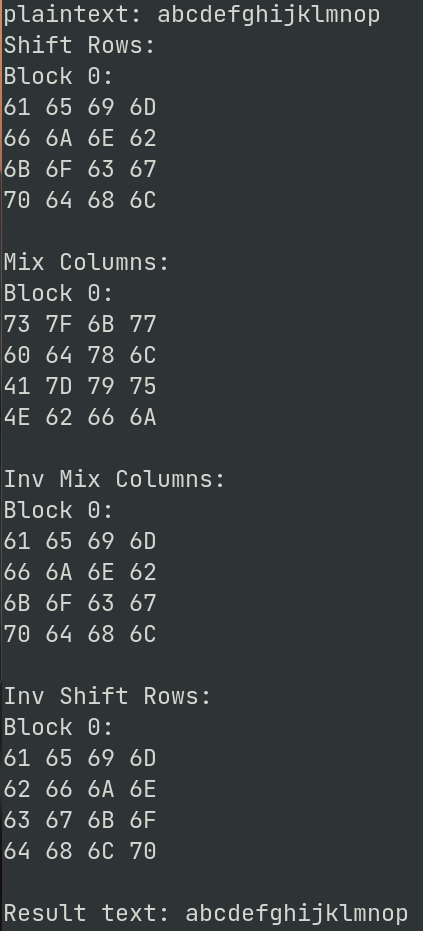
\includegraphics[width=.3\linewidth]{aes_t2.png}
  \caption{行移位变换和列混合运行结果}
  \label{fig:t2}
\end{figure}

\section{轮密钥生成}

\subsection{轮密钥生成算法}

为了把一个 128 bits 的密钥扩展到 AES128 的 10 轮迭代中,我们需要使用密钥扩展算法。
其实 AES 的密钥扩展比较简单,仍然使用的是字节循环右移(4个字节构成一组,或者说 state 中的一列)和 SBOX 的直接替换来实现的。
在最后还要再加上(异或) RCON 中规定的 $GF(2^8)$ 多项式。

代码实现如下,

  \begin{minted}[texcomments,tabsize=2,fontsize=\footnotesize,style=friendly,bgcolor=friendlybg]{rust}
fn key_schedule(cipher_key: &[u8; BLOCK_SIZE]) -> [u8; (ROUND + 1) * BLOCK_SIZE] {
    let mut round_keys = [0u8; (ROUND + 1) * BLOCK_SIZE];
    for i in 0..BLOCK_SIZE { round_keys[i] = cipher_key[i]; }
    for i in 1..(ROUND + 1) {
        // last 4 bytes (one word), i.e., last column
        let mut temp_offset: usize = i * 16 - 4;
        // last round (16 bytes), i.e., last round key
        let mut last_round: usize = (i - 1) * 16;
        // RotByte is cyclic right shift, e.g., (a, b, c, d) => (b, c, d, a)
        round_keys[i * 16] = sub_byte(round_keys[temp_offset + 1]) ^ RCON[i] ^ round_keys[
            last_round + 1];
        round_keys[i * 16 + 1] = sub_byte(round_keys[temp_offset + 2]) ^ round_keys[
            last_round + 2];
        round_keys[i * 16 + 2] = sub_byte(round_keys[temp_offset + 3]) ^ round_keys[
            last_round + 3];
        round_keys[i * 16 + 3] = sub_byte(round_keys[temp_offset]) ^ round_keys[
            last_round];
        for j in 1..4 {
            temp_offset += 4;
            last_round += 4;
            round_keys[i * 16 + j * 4] = round_keys[last_round] ^ round_keys[temp_offset];
            round_keys[i * 16 + j * 4 + 1] = round_keys[last_round + 1] ^ round_keys[
                temp_offset + 1];
            round_keys[i * 16 + j * 4 + 2] = round_keys[last_round + 2] ^ round_keys[
                temp_offset + 2];
            round_keys[i * 16 + j * 4 + 3] = round_keys[last_round + 3] ^ round_keys[
                temp_offset + 3];
        }
    }
    round_keys
}
\end{minted}

\subsection{运行结果}

使用原始密钥'abcdefghijklmnop'生成总计11组扩展密钥,将用于之后的加解密。初始密钥K转换为字节矩阵后的4列为 $W\_0 \sim W\_3$,后续的 $W\_4 \sim W\_{43}$ 使用递归计算得到。
计算结果如图~\ref{fig:t3}所示。

    \begin{figure}[h]
\centering%
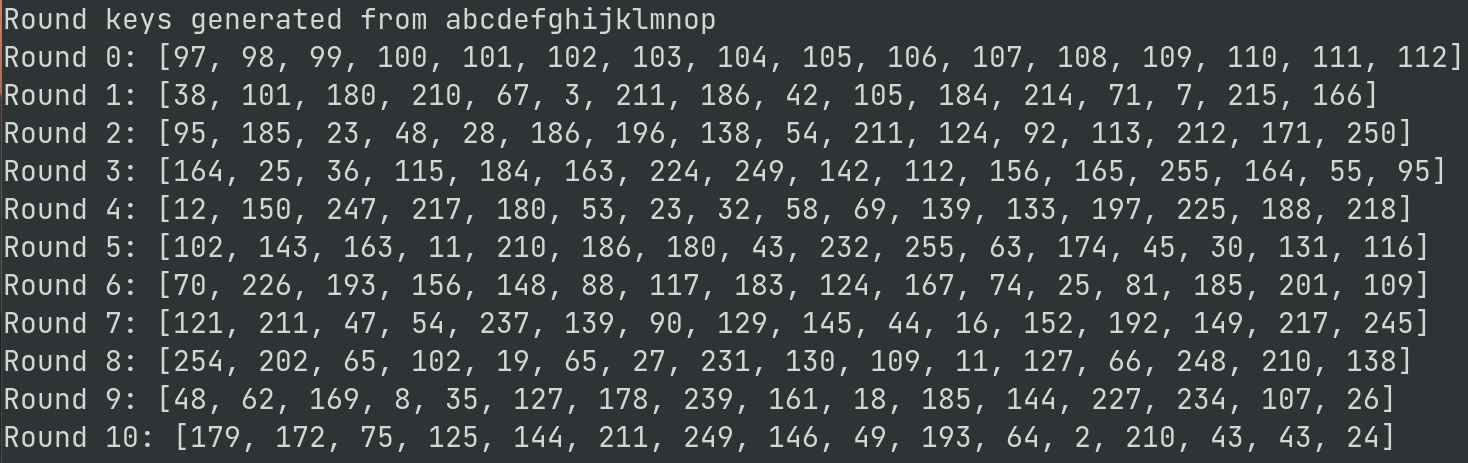
\includegraphics[width=\linewidth]{aes_t3.png}
  \caption{轮密钥生成运行结果}
  \label{fig:t3}
\end{figure}

\end{document}
